%----------------------------------------------------------------------------------------
%	PACKAGES AND DOCUMENT CONFIGURATIONS
%----------------------------------------------------------------------------------------
\documentclass[11pt]{article}
\usepackage{amsmath} % Required for some math elements
\usepackage{hyperref} 
\usepackage{xcolor}
\usepackage{lipsum} 
\usepackage{cite}
\usepackage{graphicx} % Required for the inclusion of images
\usepackage{algorithmic}
\usepackage{array}
\usepackage{bookmark}
\usepackage{listings}
\usepackage{amssymb}
\usepackage{enumitem}
\usepackage{pythonhighlight}
\usepackage[T1]{fontenc}
\usepackage{inconsolata}
\usepackage[margin=8mm]{geometry}
\usepackage[caption=false, font=footnotesize]{subfig}
\usepackage{fancyhdr}
\pagestyle{fancy}
\renewcommand{\headrulewidth}{0.4pt}
\renewcommand{\footrulewidth}{0.4pt}

\usepackage[active,tightpage]{preview}
\renewcommand{\PreviewBorder}{1in}
\newcommand{\Newpage}{\end{preview}\begin{preview}}
  


\newlist{steps}{enumerate}{1}
\setlist[steps, 1]{label = Step \arabic*:}

\hypersetup{ %color attributes of citation, link, etc.
    colorlinks=true,
    linkcolor=blue,
    filecolor=gray,      
    urlcolor=blue,
    citecolor=blue,
}

\newcommand{\matlab}{\textsc{Matlab }} %very important and totally necessary addition
\newcommand{\hdotrule}[1]{\hbox to \textwidth{\leaders\hbox to #1pt{\hss . \hss}\hfil}}

\newcommand\Item[1][]{%
  \ifx\relax#1\relax  \item \else \item[#1] \fi
  \abovedisplayskip=0pt\abovedisplayshortskip=0pt~\vspace*{-\baselineskip}}
%----------------------------------------------------------------------------------------
%	DOCUMENT INFORMATION
%----------------------------------------------------------------------------------------

\title{ECEN 405 \\ Lab 3: Power converters \\ (Part 3 - Boost converter) Submission}
\author{Daniel Eisen : 300447549}
\date{\today}

\begin{document}
\begin{preview}

    \maketitle
    \hrule
    %----------------------------------------------------------------------------------------
    %	DOCUMENT CONTENT
    %----------------------------------------------------------------------------------------
    \section{Calculations}
    $$\mathrm{\textbf{Constants:}} \; V_{d}=20V, R_L=500, D=0.3, L=4mH, C=100\mu F$$

    \subsection*{Output Voltage}
    $$V_o = \frac{D}{1-D}V_d = 30V$$

    \subsection*{Output Current}
    $$I_{o}=\frac{V_{o}}{R_{L}} = 0.06A$$

    \subsection*{Inductor Current Ripple}
    $$I_{ripple}=0.2I_{o}\frac{V_{o}}{V_{d}} = 0.018A$$

    \subsection*{Switching Frequency}
    $$f_{sw}=\frac{V_{d}\left(V_{o}-V_{d}\right)}{LI_{ripple}V_{o}} = 92592.5925926 \approx 92.59kHZ$$

    \subsection*{Output Voltage Ripple}
    $$V_{ripple}=\frac{I_{omax}D}{f_{sw}C}$$
    $$I_{omax}=I_{o}+0.5I_{ripple}=0.069A$$
    $$V_{ripple}=0.002484 \approx 2.5mV$$

    \section{\textit{Drain} of MOSFET}
    \begin{center}
        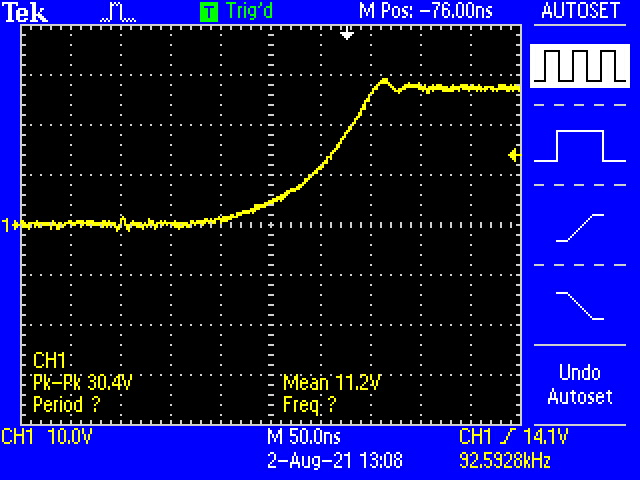
\includegraphics[width=0.35\textwidth]{img/rising.JPG}
        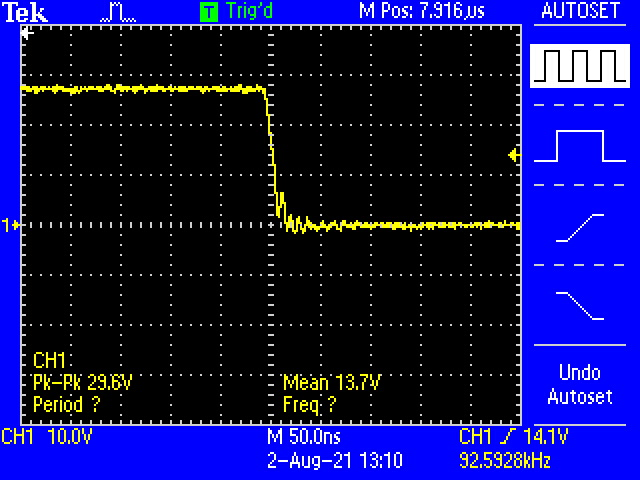
\includegraphics[width=0.35\textwidth]{img/falling.JPG}

        \textit{Fig 1. Rising Edge and Falling Edge}
    \end{center}

    At the MOSFET the boosted 30V PWM waveform is seen, with a frequency of 92.59kHz. Worthy of note is the diffents in edges, with a slow rise and slight ringing on fall.
    
    \section{Efficiency vs Output Current}
    \begin{center}
        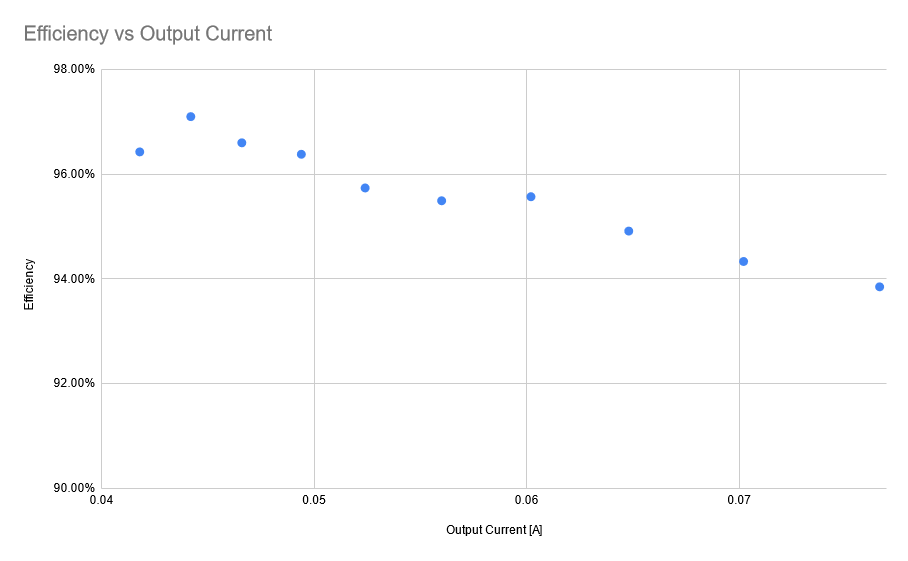
\includegraphics[width=0.5\textwidth]{img/eff.png}
        
        \textit{Fig 2. Efficiency vs Output Current}
    \end{center}
    \hrule
\end{preview}
\end{document}